\documentclass{sig-alternate}
  \pdfpagewidth=8.5truein
  \pdfpageheight=11truein

\begin{document}
%
% --- Author Metadata here ---
\conferenceinfo{SAC'13}{March 18-22, 2013, Coimbra, Portugal.}
\CopyrightYear{2013} % Allows default copyright year (2002) to be over-ridden - IF NEED BE.
\crdata{978-1-4503-1656-9/13/03}  % Allows default copyright data (X-XXXXX-XX-X/XX/XX) to be over-ridden.
% --- End of Author Metadata ---
 
\title{Non-Functional Requirements for Service-Based Applications : A Systematic Review}

% \subtitle{[Extended Abstract]
% \titlenote{A full version of this paper is available as
% \textit{Author's Guide to Preparing ACM SIG Proceedings Using
% \LaTeX$2_\epsilon$\ and BibTeX} at
% \texttt{www.acm.org/eaddress.htm}}}
%
% You need the command \numberofauthors to handle the 'placement
% and alignment' of the authors beneath the title.
%
% For aesthetic reasons, we recommend 'three authors at a time'
% i.e. three 'name/affiliation blocks' be placed beneath the title.
%
% NOTE: You are NOT restricted in how many 'rows' of
% "name/affiliations" may appear. We just ask that you restrict
% the number of 'columns' to three.
%
% Because of the available 'opening page real-estate'
% we ask you to refrain from putting more than six authors
% (two rows with three columns) beneath the article title.
% More than six makes the first-page appear very cluttered indeed.
%
% Use the \alignauthor commands to handle the names
% and affiliations for an 'aesthetic maximum' of six authors.
% Add names, affiliations, addresses for
% the seventh etc. author(s) as the argument for the
% \additionalauthors command.
% These 'additional authors' will be output/set for you
% without further effort on your part as the last section in  
% the body of your article BEFORE References or any Appendices.

\numberofauthors{5} %  in this sample file, there are a *total*
% of EIGHT authors. SIX appear on the 'first-page' (for formatting
% reasons) and the remaining two appear in the \additionalauthors section.
%
\author{
% You can go ahead and credit any number of authors here,
% e.g. one 'row of three' or two rows (consisting of one row of three
% and a second row of one, two or three).
%
% The command \alignauthor (no curly braces needed) should
% precede each author name, affiliation/snail-mail address and
% e-mail address. Additionally, tag each line of
% affiliation/address with \affaddr, and tag the
% e-mail address with \email.
%
% 1st. author
\alignauthor Valeria de Castro\\
       \affaddr{Universidad Rey Juan Carlos}\\
       \affaddr{M\'{o}stoles, Spain}\\
       \email{Valeria.deCastro@urjc.es}
\alignauthor
       Martin A. Musicante\\
       \affaddr{Federal University of Rio Grande do Norte (UFRN)}\\
       \affaddr{Natal-RN, Brazil}\\
       \email{mam@dimap.ufrn.br}
\alignauthor
       Umberto Souza da Costa\\
       \affaddr{Federal University of Rio Grande do Norte (UFRN)}\\
       \affaddr{Natal-RN, Brazil}\\
       \email{umberto@dimap.ufrn.br}        
\and
\alignauthor
       Pl\'acido A. Souza Neto\\
	   \affaddr{Federal Institute of Rio Grande do Norte (IFRN)},\\
       \affaddr{Natal-RN, Brazil}\\
       \email{placido.neto@ifrn.edu.br}
\alignauthor Genoveva Vargar-Solar\\
       \affaddr{French Council of Scientific Research}\\
       \affaddr{LIG-LAFMIA }\\
       \affaddr{Saint Martin d'H\`{e}res, France}\\
       \email{Genoveva.Vargas-Solar@imag.fr}
}
% There's nothing stopping you putting the seventh, eighth, etc.
% author on the opening page (as the 'third row') but we ask,
% for aesthetic reasons that you place these 'additional authors'
% in the \additional authors block, viz.
\date{21 September 2013}
% Just remember to make sure that the TOTAL number of authors
% is the number that will appear on the first page PLUS the
% number that will appear in the \additionalauthors section.


\maketitle
\begin{abstract}
This paper presents a systematic literature review of non-functional
requirements (NFRs) for service-based applications. 
We propose the classification of non-functional requirements into 3 levels:
\textit{business}, \textit{service} and \textit{system}. 
During the development process, the NFRs can be refined from 
one level to a more concrete level (\textit{i.e.}, from business to service
level or from service to system level). Along with the classification, we also
propose a specific nomenclature for this type of modelling. 
\end{abstract}

% A category with the (minimum) three required fields
%\category{H.4}{Information Systems Applications}{Miscellaneous}
%A category including the fourth, optional field follows...
%\category{D.2.8}{Software Engineering}{Metrics}[complexity measures,
%performance measures]

%\terms{Delphi theory}

\keywords{Non-functional requirements, Classification, Sevice-based
development, Contraints, Contract, Policy}

\section{Introduction}

Non-functional aspects concerning services and applications semantics are often
expressed as requirements and constraints.
It is not uncommon to these aspects not not to be fully considered during the development of applications.
In many cases, they are considered once the
application has been implemented, in order to ensure some
level of reliability (e.g., data privacy, exception handling,
atomicity, data persistence). 
This situation leads to service-based
applications that are partially specified and that are thereby
partially compliant with their requirements. 

In systems and requirements engineering, a non-functional
requirement (NFR) specifies criteria about the behaviour of a
system. 
These criteria may be not related to the results produced by the system,
but to other conditions of its performance. 
Non-functional requirements are often called qualities of a system. 
They are also referred as ``constraints'', ``quality attributes'', ``quality goals'', ``quality of
service requirements'' and ``non-behavioural requirements'' \cite{Stellman2005}. 
In the case of service-based applications, non-functional requirements concern
the application itself as well as its component services. 
 
As services are independent components, ensuring non-functional properties is a
challenge.
Different
studies~\cite{Babamir2010,AgarwalLS09,CholletL09,GutierrezRF10,XiaoCZBOLH08,JeongCL09,TsadimasNA12}
try to associate non-functional requirements to services using different approaches. 
Associating non-functional requirements to services
compositions can help to ensure that the resulting application is compliant to
the user requirements and also with the characteristics of the services it uses.
 
%  in developing this type of application. To adapt quality properties in
% the web service development context can provide a greater software reuse.


 Attempts to solve these problems have led to the development of a great deal of
 work in non-functional attributes and non-functional requirements. Although
 they are used as synonyms in most NFR approaches \cite{MairizaZN10}, we will
 distinguish the concepts of non-functional requirements and non-functional attributes.
 NFRs will be defined as a group of semantically correlated
 non-functional attributes (NFA). For example, \textit{security} is an
 non-functional requirement that comprises attributes such as
 \textit{confidentiality} and \textit{integrity}. A non-functional
 attribute describes the characteristics of a functional requirement. 
 
In this context, this paper presents \textit{(i)} a systematic review
 of the treatment given to non-functional requirements for web service based applications, and
 \textit{(ii)} proposes a classification of the non-functional requirements for
these kind of applications.
 
% The goal of this chapter is presents, based the concepts obtained from
% non-functional requirements and software engineering methodologies' works,
% a systematic analysis concerning \textit{(i) a towards NFR
% classification for reliable web service development, (ii) its application on the modeling web services composition and
% (iii) how to apply these set of concepts through a proposal for a reliable web
% service based methodology development}. 
 
The analysis will be conducted in the form of a systematic review
%\footnote{A systematic review provides means of identifying,
% evaluating, and interpreting the literature relevant to a particular research
% question or topic area} 
\cite{Kitchenham08}.
 The result of this review can be useful to summarize the existing treatment of NFRs and to provide a background to new research activities.
 
%  We present an analysis into 2 parts to facilitate the understanding of the
%  areas and related works and what their importance in the context of
%  service-based development.  Our goal is to identify a common nomenclature for existing NFR
%  and web service based methodologies and propose a specification of these
%  concepts in the context of reliable web services development. 
%  
%  Since the focus of this work is the development of reliable service-based
%    applications, we analyzed what are, where and how non-functional requirements
%    are modeled in the development of this type of application. Allied to this,
%    we analyzed which methodologies aim the development of service, and if
%    consider modeling of non-functional aspects. 

The paper is organized as follow: Section \ref{sec:nfrs} presents a systematic
literature review of non-functional requirements for service-based application.
In Section \ref{sec:classification} we propose a classification of the NFRs
considering the analysis of works made in the systematic review section. Section
\ref{sec:conclusion} concludes the paper.
   
\section{Non-Functional Requirements\\ for Service-Based Applications}   
\label{sec:nfrs}   

This section presents a systematic review of the non-func\-tion\-al
requirements and properties used in the context of service-oriented
development. The purpose of our analysis is:
\begin{itemize}
  \item to identify the concepts, properties and notations used in the
  service-based systems development;
  \item to find if there is any pattern or relationship between non-functional
requirement concepts in different modelling levels.
\end{itemize}

For each phase of the development, the requirements and non-functional
requirements are refined. As a result of this process, the granularity of the
concepts described by the requirement becomes thinner and more precise. 

% The focus of a modeling-based non-functional requirements becomes important
% because it reveals a continuing need on the development of distributed
% service-oriented. Thus, it is necessary identify how non-functional requirements
% are classified in different development process phases and iterations.

% Thus, this section also presents the collected data and results
% from the research work analysis according to some research questions. Once the
% sources' extraction execution had been completed, it was important to be sure
% that multiple publications of the same approach were not included in the data analysis. Tables \ref{tab:result02}
% and \ref{tab:result03} show the results of each work under each question
% described in section \ref{subsec:question}.  





% % Among the properties presented we highlight the security
% % and performance properties. All users want to access data
% % securely and quickly. Most studies analyzed have both properties. Reliability is
% % also an important non-functional requirement presented in some papers and needed
% % to end users. 

% 
% The analisys was carried out by effectuating the following activities:
% \textit{(i) question formulation; (ii) source selection; (iii) selection
% process; (iv) information extraction;} and \textit{(v) results}.

We propose 7 research questions ($RQ_1$ to $RQ_7$) to guide our analysis about non-functional
requirements. 
For each question we define a set of possible answers in order to guide
the analysis.
These possible answers are defined from our knowledge on each topic. 
The questions are closely related to service-oriented development with a NFR focus.
They are:
\begin{itemize} 
  \item \textbf{\texttt{$RQ_1$:}} How are NFR modelled by existing
  methodologies for developing reliable Web services?
  \begin{itemize}
	  \item \textit{Answer is specific to each proposal}
	\end{itemize}  
 \item \textbf{\texttt{$RQ_2$:}} Which are the NFR that are more frequently
 by methodologies developing web services?
 	\begin{itemize}
	  \item \textit{Possible answers: security / availability / portability / \ldots / reliability /
	  performance}
	\end{itemize}
  \item \textbf{\texttt{$RQ_3$:}} What is the software
  development approach used in the paper?
	\begin{itemize}
	  \item Possible answers: \textit{Model driven approach (*MDD) / Ontology (*Ont) / Formal method
	  (*FM) / Artificial intelligence (*AI) / Business Process Modeling (*BP)
	  Traditional (*TDT)}
	\end{itemize} 
  \item \textbf{\texttt{$RQ_4$:}} What is the discipline (application domain)
  of the ``\textit{non-functional requirements}'' / ``\textit{non-functional
  properties}'' used in the work?
  \begin{itemize}
	  \item Possible answers: \textit{Software architecture / QoS model / Language definition /
	  Methodology / etc}
	\end{itemize}	
  \item \textbf{\texttt{$RQ_5$:}} Does the paper proposes a (meta)model
  describing and analyzing NFR? Is there any relationship between
  the non-functional requirements (meta)model proposed and business services? 
\begin{itemize}
	  \item Possible answers: \textit{yes / no} -- \textit{yes / no}
	\end{itemize}  
  \item \textbf{\texttt{$RQ_6$:}} Do the non-functional aspects are treated in
  an independent way?
\begin{itemize}
	  \item Possible answers: \textit{single / composition}
	\end{itemize}
\item \textbf{\texttt{$RQ_7$:}} Which is the publication year of the paper?
	\begin{itemize}
	  \item Possible answers: \textit{Year of publication}
	\end{itemize}	   
\end{itemize}


% \subsection{Source Analysis}
% \label{subsec:souce_analysis}

% In the development of systems, for each phase of development,
% the requirements are being refined and the granularity becomes tiner after each
% iteration. With the analysis, we can identify how these NFRs have been
% classified.
 
The research questions identify characteristics
 of the ser\-vice-oriented application development, especially the
modelling of non-functional requirements/properties, how they are addressed and
if there is any classification.   

\bigskip

We used the approach described in \cite{Kitchenham08} for searching,
collecting and selecting works related with non-functional requirements for
developing service-based applications. Based on these data we analyzed concepts used
in each work for the description of NFRs and the difference among them. 

We selected the sources proposed by \cite{Kitchenham08} for searching primary
studies. These sources contain the works published in journals, conferences and
workshops which are of recognized quality within the research community. The
search engines are: \textit{(i) IEEE Computer; (ii) ACM Digital Library;} and
\textit{(iii) Science Direct}. In the selected sources, we used the following search
query criteria:

\begin{center}
\texttt{(((non functional properties) OR (non functional requirements))
AND web service AND composition))}
\end{center}


After define the sources' selection, we apply the
process used to identify those works that provided direct
evidence with regard to the research questions. Deciding
for the inclusion and exclusion criteria for filtering the corpus works
selection, we selected those related to non-functional requirements/properties,
and quality for web service based applications. Initially, the selection
criteria were interpreted liberally and clear exclusions were only made with
regard to title, abstract and introduction.

Based on the guidelines mentioned in \cite{Kitchenham08}, we established a
multi-step process made up of three steps with different selection
criteria:

\begin{itemize}
\item Step 1 - the search string must be run on the selected
search engine. An initial set of studies was obtained by filtering
of title, abstract, and if necessary, introduction. All the studies were
selected according to the inclusion and exclusion criteria. Studies which
were not clearly related to any aspect of the research questions
were excluded.
\item Step 2, the exclusion criteria were based on the following
practical issues: non-English papers, non-
International Conference papers and non-International Workshop
papers. Specifically in the case of ACM library, we considered only the
transaction journal works.
\item Step 3, the papers selection process was based on detailed
research questions.
\end{itemize}

The information for each step was collected considering the 3 searchers
and the the query presented previously. the results of each step were:
\textit{(i)} for each source a list of all the studies that
fulfilled the query; \textit{(ii)} a list
of studies for each source which contained all the works that did not fulfill the
second stage inclusion criteria; and
\textit{(iii)} the last step produced a list of works for each source which
contained all the studies that fulfilled the second step.


The notation used to refer non-functional requirements will be highlighted in
\textit{italic}, as well as the set of values that can be associated with each
concept. For example, a notation used by a work can be \textit{quality property}
or \textit{non-functional concern}, and the values associated with
its notation are \textit{security}, \textit{reliability}, \textit{transaction},
etc. Thus, considering the research question, we analyze a set of works in order
to identify any pattern or divergence between the analyzed literature. 

\bigskip

Babamir et al.\cite{Babamir2010} ranks services \textit{quality properties}
in three categories (business level, service level, system level).
\textit{Quality properties} are associated with \textit{quality constraints},
that are defined as assertions or propositional logic formulas.
\textit{Non-functional attributes, composition mo\-del entity} and \textit{mo\-del entity} are the notations used by
Xiao et al. \cite{XiaoCZBOLH08} for classifying the different concepts for
non-functional requirements modeling. Non-functional attributes (NFAs) describe
the non-function aspects in the abstract process models. The framework to
model NFRs proposes to annotate composition models with NFAs.

D'Ambrogio \cite{DAmbrogio06} uses the term \textit{quality characteristics}
to group similar characteristics into \textit{quality categories}. Each
\textit{quality characteristic} is quantified by \textit{quality dimensions}.
\textit{Quality characteristic} is a quantified QoS aspect, for example
\textit{latency, throughput, reliability, availability}, etc. \textit{Quality
characteristics} of a common subject are grouped into abstract \textit{quality
categories}, for example \textit{performance} (for latency and throughput characteristics) and
\textit{dependability} (for reliability and availability characteristics).  
 
The terms \textit{category, sub-category}
and \textit{property}  are used by Yeom
et al.\cite{Yeom2006} to classify non-functional requirements.
\textit{Business}, \textit{service} and \textit{system} are the possible values to be associated
with the proposed terms, and a \textit{sub-category} can be \textit{security,
value, interoperability}, etc. The work in \cite{Yeom2006} defines a \textit{web
services quality model}, which considers non-functional properties in several
aspects. In this model, web services qualities are classified in categories and
sub-categories. Chollet et al.\cite{CholletL09} uses only two terms to
classify and relate quality properties with services, they are:
\textit{activity} and \textit{quality property}. Each activity represents a
functional property that can be divided in sub-activities, depending on its
granularity. For non-functional requirements, the work in \cite{CholletL09}
describes the possibility of creating different meta-models for each
\textit{quality property}, and then relate them with activities.   


Schmeling et al.\cite{SchmelingCM11} uses the 
\textit{non-functional concerns (NFC)} notation to describe NFRs. This term
encompasses two aspects: the specification of NFCs and their realization.
\cite{SchmelingCM11} defines that a \textit{functional concern (FC)} is a
consistent piece of functionality that is part of a software system.
\textit{Non-functional concern (NFC)} is a general term describing a matter of interest or importance that does correspond
to a non-functional requirement of a system, for example, \textit{security,
reliability, transactional behavior}, etc. A \textit{non-functional action} represents some
behavior that results in a \textit{non-functional attribute}. An example of
\textit{non-functional action} is \textit{encryption}, which realizes the \textit{non-functional attribute},
\textit{confidentiality}. A \textit{non-functional activity} is also used as a
term, which means to encapsulate the control flow of \textit{non-functional
action} that apply to the same subject. The term is used in analogy to activity
and action in UML2.

Ceri et al.\cite{CeriDMF07} uses the terms \textit{policy, rule,
condition} and \textit{action model} to specify NFRs, and in a similar way,
Agarwal et al.\cite{AgarwalLS09} also uses the concept of \textit{service
policy} associated with the concept of service. Each service is also associated
with a \textit{service property}, which may have a specific value
(\textit{security, reliability}, and so on). Each service is also associated
with a \textit{unit function}, that represents one or more
requirements.

Ovaska et al.\cite{OvaskaEHPA10} uses
\textit{quality attribute, category, conceptual layer} and \textit{importance}
to organize and classify the NFRs, Pastrana et al.\cite{PastranaPK11} uses
the term \textit{contract} to describe non-functional requirements. In a
\textit{contract} it is possible to define pre-conditions, post-conditions and
invariants. A \textit{web service} can have many \textit{contracts}, that
defines many \textit{assertions} and are associated with \textit{quality
properties}. 




Some related papers do not have any
nomenclature to classify non-functional requirements. However, some of them uses
the \textit{attribute} notation \cite{ZhangPSP05,BasinDL06,JeongCL09}, other
uses \textit{properties} \cite{Fabra2011}, other \textit{factors}
\cite{MohantyRP10,GutierrezRF10}, \textit{characteristics}
\cite{DiamadopoulouMPS08}, \textit{quality level} \cite{ModicaTV09} or
\textit{values} \cite{ThissenW06,BasinDL06}.


\subsection{Analysis}
\label{sec:proposal}

% The purpose of this analysis is to identify the properties and non-functional
% requirements used in the development of systems, looking for patterns
% or relationships between non-functional concepts in different
% modeling levels.

Although there exist many different types of notation used for classify
non-functional requirements, in general, the values associated to them are the
same, \textit{i.e.} \textit{security, performance, reliability, usability, availability}, etc. What
distinguishes the different approaches is the adoption of different NFR
hierarchies in order to prioritize or classify the quality requirements. 
Another interesting factor
is that the each work uses different approaches to model these requirements.
Thus, there are different kinds of notations for non-functional
requirements.

  
\begin{table*}[ht!]
\centering
%\scriptsize
\tiny
\begin{tabular}{l|l|l|l|l}
  \hline 
  \hline
   \textbf{Reference} & \textbf{\textit{NFR concepts}} &
   \textbf{\textit{NFR values}} & \textbf{\textit{Approach}} &
   \textbf{\textit{Domain / Scope}} 
   \\
  \hline
  \hline  
  Babamir et al. \cite{Babamir2010} &  property / & responsiveness /
  availability   & TDT & Software architecture
 \\  
  & category /  & performance / sla properties   &  & 
 \\
 &  constraint &    &  & 
 \\ 
  \hline   
 
  Yeom et al. \cite{Yeom2006} & category / & business value / performance /
   & TDT & QoS model\\ 
   & sub-category / & stability /manageability /   & & \\
   & property & security / business processing  & & \\
    &  & interoperability & & \\ 
  \hline 
  
  Xiao et al. \cite{XiaoCZBOLH08} &  NF attribute  & time /
cost / resource  & BP  & Business processes
   \\
 	&   &   &  & modeling
   \\   
  \hline 
  D'Ambrogio \cite{DAmbrogio06} &  characteristics /  & availability /
  reliability / & MDD & WSDL \\ &  category /  &  access control  &  &
  extension
  \\
  &  dimension &    &  & 
 \\
   \hline
  Chollet et al. \cite{CholletL09} & activity / & security  & MDD 
  & Orchestration Framework
   \\
  &  NF attribute &    &  & 
  \\
  
  \hline
  Schmeling et al. \cite{SchmelingCM11} & NF concern / & security &
  MDD &  Web service 
  \\
  & NF attribute / &  &
   & composition process
    \\
  &  NF action / &    &  &
   \\
  &  NF activity	 &    &  &
  \\ 
  \hline
    Thi{\ss}en et al. \cite{ThissenW06} & NF value  &  performance /
  reliability &  FM & Software architecture \\  
   & & cost / availability &  & \\  
  \hline
  Zhang et al. \cite{ZhangPSP05} & attribute /& security & FM &  Access control 
   \\
  &  predicate &    &  &
  \\
  
  \hline
  Basin et al. \cite{BasinDL06} &  attribute & security  & MDD & System
  architecture
  \\
  \hline
  Ceri et al. \cite{CeriDMF07} & police / rule  & n.a. & TDT & Context-aware
  applications
   \\
  &  condition / action &    &  &
  
  \\
  \hline
  Fabra et al. \cite{Fabra2011} & property & storage /
  processing & MDD & Web service methodology 
  \\
   &   & (*case study) &  & 
  \\
  \hline
  Modica et al. \cite{ModicaTV09} & quality level & sla
  properties & TDT &  Service oriented 
  \\
   &  &  &  & architecture \\
  \hline
  Ovaska et al. \cite{OvaskaEHPA10} & attribute & security / reliability
  & MDD &  Model development
  \\
   
  &  category &    &  &
  \\
  \hline
  Agarwa et al. \cite{AgarwalLS09} & property / & \textit{not explicitly
  defined} & Ont & Policy language
  \\
   
  &  policy / &    &  &
  \\
  
  &  function &    &  &
  \\
  \hline
   &  & operation cost /&  &  \\
  &  & performance / availability /  &  &  \\
  Jeong et al. \cite{JeongCL09} & NF attribute & accessibility / security /
  & AI  & Service oriented   \\ 
   &  &
  interoperability / usability / & & \\ &  & user satisfaction &  & architecture
  \\
  \hline
   &  & performance / reliability /  &  & \\
   & NF property / & scalability / capacity /&  & \\
  Pastrana et al. \cite{PastranaPK11} & contract  / & robustness /
  precision / & Ont & Web service methodology\\
  & assertion / & accessibility
  / availability / &  & \\ 
   & NF behaviour & interoperability / security  &  & \\    
  \hline
  Diamadopoulou et al. \cite{DiamadopoulouMPS08} & NF characteristic &
  user' subjective & TDT & Web service selection  \\ 
   &  & perception  & &  \\
  \hline
  Gutierrez et al. \cite{GutierrezRF10} & NF factor & Security  & BP &  Web
  service
  \\
   &  NF sub-factor&   &  &  development process
  \\  
  \hline
  Mohanty et al. \cite{MohantyRP10} & NF attribute or & reliability /
  performance / & & Artificial intelligent /\\ 
  & NF factor & integrity / usability  & AI  & Web services classification	 \\
  &  & response time / documentation &   &  \\
  
  \hline  
  \hline  
\end{tabular} 
\caption{Research question results - $RQ_1$, $RQ_2$, $RQ_3$, $RQ_4$.}
\label{tab:result02}
\end{table*} 
 
A number of approaches use
\cite{DAmbrogio06,CholletL09,SchmelingCM11,BasinDL06,Fabra2011,OvaskaEHPA10} MDD
(Model Driven Development) for designing and developing systems. Fabra
\textit{et al.} \cite{Fabra2011} presents a complete methodology that does not
mainly focus on non-functional requirements. Fabra \textit{et al.} \cite{Fabra2011} also describes the importance of the use of MDD in the development of
service-oriented applications. \cite{ThissenW06,ZhangPSP05} use formal methods
to define a development process based on NFR for web services,
\cite{AgarwalLS09,PastranaPK11} use ontologies for the definitions and
modeling of non-functional requirements and \cite{XiaoCZBOLH08,GutierrezRF10} use Business Process Modeling (BPM) for
system specification, including NFR. Most works focus on composition
service modeling while others define requirements models to
represent the properties used.

In \cite{Babamir2010,Yeom2006} non-functional properties for web services
are classified into three categories such as
\textit{service level view, system level view} and \textit{business level view}.
In the \textit{\textit{business}} level the quality properties are:
\textit{service charge, compensation rate, penalty rate} and
\textit{reputation}; at the \textit{\textit{service}} level the quality
properties are: \textit{performance} and \textit{stability}; and at the
\textit{system} level the quality properties are classified into:
\textit{manageability, interoperability, business processing} and
\textit{security}.

In the method defined in \cite{XiaoCZBOLH08}, each task in the process model is
annotated with the NFAs (\textit{non-functional attributes}). During the design phase, the
service composition and the definition of NFAs are separated. Then,
each task in the process model is annotated with the corresponding NFA. The
attributes are related with tasks or data item. For data, the NFAs are:
\textit{value} and \textit{range}; and for tasks the NFAs are: \textit{cost,
time, resources} and \textit{expression}.

D'Ambrogio \cite{DAmbrogio06} presents a WSDL extension for describing the QoS
of web services. The process is based on MDA. The work presents a catalog
of \textit{QoS characteristics} for the web service domain and the Q-WSDL
(Quality WSDL) meta-model for modeling QoS properties in web services. The properties
presented are: \textit{availability, reliability} and \textit{access
control}. \cite{CholletL09} presents a security meta-model for web service
composition. The non-functional requirements considered concern
\textit{authentication, integrity} and \textit{confidentiality}. Each property is related with a service activity. In \cite{SchmelingCM11}, authors
present an approach and a toolset for specifying and implementing the
composition of several non-functional properties of Web services. The
non-functional attributes described in \cite{SchmelingCM11} are: \textit{confidentiality, integrity
(security concern)} and \textit{response time (performance concern)}.

The work presented in \cite{ThissenW06} describes
steps to design a selection mechanism of services identified as candidates for
participating in a composition, considering their quality properties. The steps
are: \textit{(i)} identification of relevant QoS information; \textit{(ii)} identification of basic composition patterns and
QoS aggregation rules for these patterns; and \textit{(iii)} definition of a
selection mechanism of service candidates. As QoS properties considered in
\cite{ThissenW06} are: \textit{performance, cost, reliability} and
\textit{availability}. 
  
% We highlight the following works: \cite{CeriDMF07, 
% Yeom2006,JeongCL09,PastranaPK11}. These research works present a relevant
% detail of some NFR and a good detail of them in each stage of development.

Among the properties presented we highlight \textit{security}
and \textit{performance}. Users usually need to access data
securely and quickly. Most studies have both properties as the most
important non-functional requirements. \textit{Reliability} is also an important
non-functional requirement presented in some works and required by end users.

We can now relate the research questions presented in section \ref{sec:nfrs},
with the works described above. Tables \ref{tab:result02} and \ref{tab:result03}
show some results.

The vocabulary used for naming and characterizing NFR is not stable, 5 works out
360 (1.6\%). 19 of the total of works chosen (26.31\%) propose a
classification of non-functional requirements.

% The many different types of NFR terms used
% in these works, there is still no clear classification of NFRs
% and a hierarchy or dependency between them. Only 5 of the works present a hierarchy
% among the different non-functional requirement notations, representing only
% 1.6\% of the total (over 306 works - appendix \ref{append:analysis}) and 26.31\% of total of
% works chosen (over 19 works - appendix \ref{append:analysis}). This hierarchy
% is used according to the modeling level and process phase. 

% Among these works, we highlight
% \cite{Yeom2006,DAmbrogio06,CeriDMF07}, because it presents the types of NFR and
% their importance at each modeling level.


 
\begin{table}[ht!]
\centering
\tiny
\begin{tabular}{l|l|l|l}
  \hline 
  \hline
   \textbf{Reference} & \textbf{\textit{Service model}} --
   & \textbf{\textit{Service type}}  &
   \textbf{\textit{Year of}} 
   \\
    &   \textbf{\textit{Business services}} &   &
   \textbf{\textit{publication}} 
   \\
  \hline
  \hline  
  Babamir et al. \cite{Babamir2010} & no -- yes  & composition & 2010   
 \\  
  \hline   
  Yeom et al. \cite{Yeom2006} & yes -- yes & single   & 2006  \\  \hline
  Xiao et al. \cite{XiaoCZBOLH08} & no -- no & composition    & 2008
   \\ 
  \hline 
  D'Ambrogio \cite{DAmbrogio06} & yes  -- no & composition  & 2006 \\
   \hline
  Chollet et al. \cite{CholletL09} & yes -- yes & composition  &  2009 \\
  \hline 
  Schmeling et al. \cite{SchmelingCM11} & no -- no & composition &  2011 \\ 
  \hline
   Thi{\ss}en et al. \cite{ThissenW06} & no -- yes & composition & 2006
   \\
  \hline
  Zhang et al. \cite{ZhangPSP05} & no -- no  & single  & 2005 \\ 
  \hline
  Basin et al. \cite{BasinDL06} & yes -- no & single / composition  & 
  2006\\
  \hline 
  Ceri et al. \cite{CeriDMF07} & no -- no  & single  &  2007\\ 
  \hline 
  Fabra et al. \cite{Fabra2011} & yes -- yes & composition  &  2011\\
  \hline
  Modica et al. \cite{ModicaTV09} & no -- no & composition & 2009\\ 
  \hline
  Ovaska et al. \cite{OvaskaEHPA10} & yes -- no & single & 2010\\
  \hline
  Agarwa et al. \cite{AgarwalLS09} & yes -- no & single / composition  &  
  2009\\
  \hline
  Jeong et al. \cite{JeongCL09} & no -- no  & composition &  2009\\
  \hline
  Pastrana et al. \cite{PastranaPK11} & yes -- no & composition &  2011 \\
  \hline
  Diamadopoulou et al. \cite{DiamadopoulouMPS08} & no -- no & composition 
  & 2008\\
  \hline
  Gutierrez et al. \cite{GutierrezRF10} & no -- no &  single / composition 
  & 2010\\
  \hline
  Mohanty et al. \cite{MohantyRP10} & no -- no  & single  & 2010\\
  \hline
  \hline  
\end{tabular}
\caption{Research question results - $RQ_5$, $RQ_6$, $RQ_7$.}
\label{tab:result03}
\end{table} 

There are other works
\cite{ieee_1998,CysneirosLN01,Cleland-HuangSZS06,Glinz05rethinkingthe,sommerville08}
that consider and propose non-functional requirements classifications. A number
of software attributes are defined as requirements in
\cite{sommerville08,ieee_1998}. According to \cite{ieee_1998}, the most common
non-functional properties are: \textit{performance}; interface; operational;
resource; verification; acceptance; \textit{maintainability}; documentation;
\textit{security}; \textit{portability}; quality; \textit{reliability};
\textit{usability}; and \textit{safety}. We highlight those that are used in
most analyzed classifications. \cite{ieee_1998} proposes an NFR specification
and a template for specifying requirements, considering both, functional and
non-functional properties.

The NFRs are classified in 4 main concepts by \cite{CysneirosLN01}. The
classification uses \textit{quality properties}. These properties are:
\textit{performance; security; cost;} and \textit{usability}. Pastrana
\cite{PastranaPK11} describes an ontology based methodology and uses a NFR
classification based in some properties, most already described in other works.
However that work is the only one to use \textit{scalability, capacity}
and \textit{precision} properties. Considering web services development,
these properties are not very frequently used, however, considering data
processing, these properties can be important in cases of large data processing
requests through services.

Sommerville \cite{sommerville08} classifies requirements,
either functional or non-functional, in three main blocks:
\textit{process, product} and \textit{external}. \cite{sommerville08} 
also defines a sub-classification considering the system domain.
Software requirements are classified as: \textit{usability; reliability; safety;
efficiency; performance;} and \textit{capacity}.  
   

% Based on the works presented in \cite{Cleland-HuangSZS06,Glinz05rethinkingthe},
% and considering the previous analysis of NFR, the properties highlighted are
% security, performance and reliability. Although the works have
% different focuses and the NFR classification and definition are made in
% accordance with different arguments, the more present in NFR ratings
% requirements are that ones presented in Figures \ref{fig:NRFmodel} and
% \ref{fig:proposalNRF}.


Some requirements may determine the system design, for example, \textit{(i)}
Keep certain functions in separate modules; \textit{(ii)} check data integrity
for critical variables; and \textit{(iii)} permit only limited communication
(requester / provider), are examples of restrictive requirements
\cite{ieee_1998}. These examples are related with some NFR concepts as: \textit{security, reliability} and
\textit{availability}. 

% Thus, in the context of service-based
% development, it is important that non-functional requirements are described
% through abstract modeling levels.
 
%    Thus, based on theses works and the
% results obteined in the systematic review, the results presented in tables
% \ref{tab:result02} and \ref{tab:result03}, we will propose a NFR model and
% classification for service based application development.
   
% \subsection{NFR Metamodel:} 
% \label{sec:servicedefinitionNFR} 


In the service-based development there is a clear difference between the
business, service and system levels. The quality requirements are treated
differently in each of these levels. Despite the different nomenclatures they
can be described in general as \textit{non-functional concern/requirement} and
\textit{non-functional attribute}.
  
Considering \cite{ieee_1998} and \cite{sommerville08}, we notice that
restrictions are usually related to use cases and functional requirements, and
in most cases, a service activity can be represented as an use case. It is in
this way that non-functional requirements with web services are related. They
don't propose a specific way to design constraints to services, but assuming
that a service is modeled as a use case, and it has quality requirements.   

At the service level, each service activity is related in some way with the
concept of contracts. Contracts can be grouped into policies and their
rules. Policies are directly related to concepts like quality,
security, performance and availability; contracts are associated with non-functional attributes. 

\bigskip

% In spite of the variety of tools and new approaches for web service development,
% there is not (yet) a consensus on a software process methodology for web
% services
% \cite{PapazoglouH06,Papazoglou03,cdl2006,MilanovicM06,FeuerlichtM05,Ramollari_asurvey,somet2005}.
% %  In order to develop and use such a methodology, it is of paramount importance to
% % provide adequate descriptions of its expected capabilities and competences.  
%  
% Works proposing methodologies can be
% classified into two types: (\textit{i}) those that propose new approaches for non-functional
% properties guarantees; and (\textit{ii}) those proposing service-oriented
% development methodologies for the whole development process.
%     
% \cite{HL05TACoS} proposes \textit{Design by Contract} for web services. It is
% possible to describe three levels for specifying contracts: \textit{implementation level,
% XML level} and \textit{model level}. Design by Contract applied to web services
% allow the verification services web through the use runtime checkers, before the
% deployment, such as \textit{jmlrac} \cite{LeavensCCRC02}, by adding behavioral
% information to the specification of services, using JML \cite{LeavensCCRC02}.
% 
% CDL (\textit{Contract Definition Language}) \cite{cdl2006} is a XML-based
% description language, for describing contracts for services. The
% development with CDL offers an architecture framework, design standards and a
% methodology \cite{MilanovicM05,Milanovic05,Milanovic06,MilanovicM06}, that can
% be easy understood and applied to the development of real applications. The
% greatest difficulty is that the language only
% represents contracts for services. Its specification is generated by
% refining B \cite{AbrialLNSS91} machines that describe
% the services and their compositions. 


% \begin{table*}
% \centering
% \caption{Some Typical Commands}
% \begin{tabular}{|c|c|l|} \hline
% Command&A Number&Comments\\ \hline
% \texttt{{\char'134}alignauthor} & 100& Author alignment\\ \hline
% \texttt{{\char'134}numberofauthors}& 200& Author enumeration\\ \hline
% \texttt{{\char'134}table}& 300 & For tables\\ \hline
% \texttt{{\char'134}table*}& 400& For wider tables\\ \hline\end{tabular}
% \end{table*}
% end the environment with {table*}, NOTE not {table}!



\begin{table}[ht!]
\tiny
\begin{tabular}{l|c|c|c|c}
  \hline
  \hline
   & IEEE & ACM  & Science Direct & Total \\
  \hline
  \hline
  Total results & 65 & 271 (75 \footnote{We considered only 75 transactions
  journal works}) & 166 & 502 (306 \footnote{considering the 75 ACM
  transactions journal works}) \\
  \hline
  Step one  & 19 & 10 & 20  & 49 \\
  Step one (\%) & 29.23\% & 13.33\% & 12\% &
  16\% \\
  \hline
  Step two & 7 & 3 & 9 & 19\\
  Step two (\%)  & 10.76\% & 4\% & 5.42\% & 6.20\%\\
  \hline
  \hline
\end{tabular}
\caption{Summary of the studies selected at each step.}
\label{tab:result01}
\end{table}


The extraction of information was based on the research questions, and each work extraction question included the following
items: \textit{(i)} where the paper was found; \textit{(ii)} identification of the title and main
subjects; \textit{(iii)} summary of the research; \textit{(iv)} inclusion and
exclusion criteria; \textit{(v)} objective and result; and \textit{(vi)}
subjective results. 


% The systematic literature review took place between December 2011 and January
% 2012 and we did not filter works within a specific year interval. Although the
% studies which were concretely analyzed were published between 2005 and 2011.
Table \ref{tab:result01} shows a summary of the studies selected in each stage
of the selection procedure for each source. The ``Total results'' were obtained
by running the search string on the selected sources. The next four rows show
the results obtained after applying stages one (2 first rows) and two (2 last
rows) of the studies selection procedure.


\begin{figure}
\centering
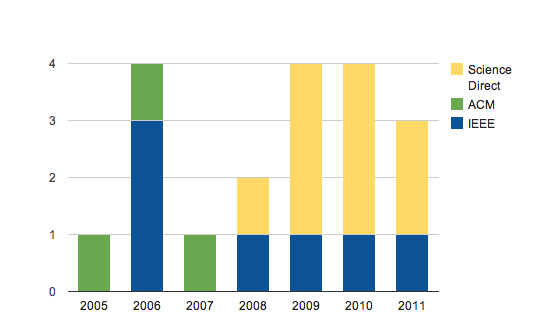
\includegraphics[width=.49\textwidth]{figs/data.png}
\caption{Publications per year.}
\label{fig:statistics}
\end{figure}


In the first step, respecting the filters described, the 65 articles collected
from IEEE, only 29.23\% of them were in accordance with the criteria
described early, representing 19 articles. In ACM Library, from 75 works
collected, only 13.33\% passed in the first stage filter, representing 10 articles. In Science Direct
had the lowest percentage, totaling 20 of the 166 articles collected by the
query, thus representing 12\% of the total. Despite being the lowest relative
value, the Science Direct had the largest absolute result, with 20 works
in the first step. In the second stage, the percentage dropped further, and the
relevant works and with accordance to the criteria have been collected as the
final result. The results were respectively, 10.76\%, 4\% and 5.42\% of total
from the IEEE, ACM and Science Direct. The highest percentage was among the
 works from  IEEE, while the largest number od results, in absolute terms,
 was collected from Science Direct. The approaches resulting from this last
 stage were studied in depth and information concerning the detailed research
 questions and other fields of the extraction forms was extracted from each
 eork we selected. 49 works were selected in the first stage, and, only 19
 works in the second stage. It represents  6.20\% of the total amount of works.


Figure \ref{fig:statistics} shows the publications per year, from
2005 to 2011. 12 of 19 articles were selected in the systematic review published
in 2006, 2009 and 2010, being four in each year and 6 in Science Direct source,
5 in IEEE, and only 1 at the ACM. All nine of Science Direct were
published in the last 4 years. Figure also
shows that the number of publications that consider classification of NFR once
again increased from 2008.



\section{Classification of Non-Functional Requirements}
\label{sec:classification}

 
According to the previous analysis, we defined the main non-functional
requirement concepts that are associated with service-based development. We also
present a synthesis of the concepts common to the analyzed approaches used for
modelling non-functional requirements of service-based applications. The NFRs
have been classified into three levels, \textit{business, services} and
\textit{systems}. According to each modeling level, non-functional requirements
are being refined from the business level to system level.

One classification of NFRs can be seen in \cite{Yeom2006}.
In that classification, NFRs are not applied on data but just to functions and
 service performance. 
We consider that it is important to classify the
 requirements of business and data (value) restrictions, since data accessible to web
 services depend on the application contexts.
  
 In sections \ref{sec:nfr-metamodel} and \ref{sec:nfr-classification} we present
 which concepts (NFR meta-model) and values (NFR classification) we consider
 important to a reasonable modeling of non-functional requirements for service
 applications.
 
 

\begin{figure*}[ht!]  
\centering  
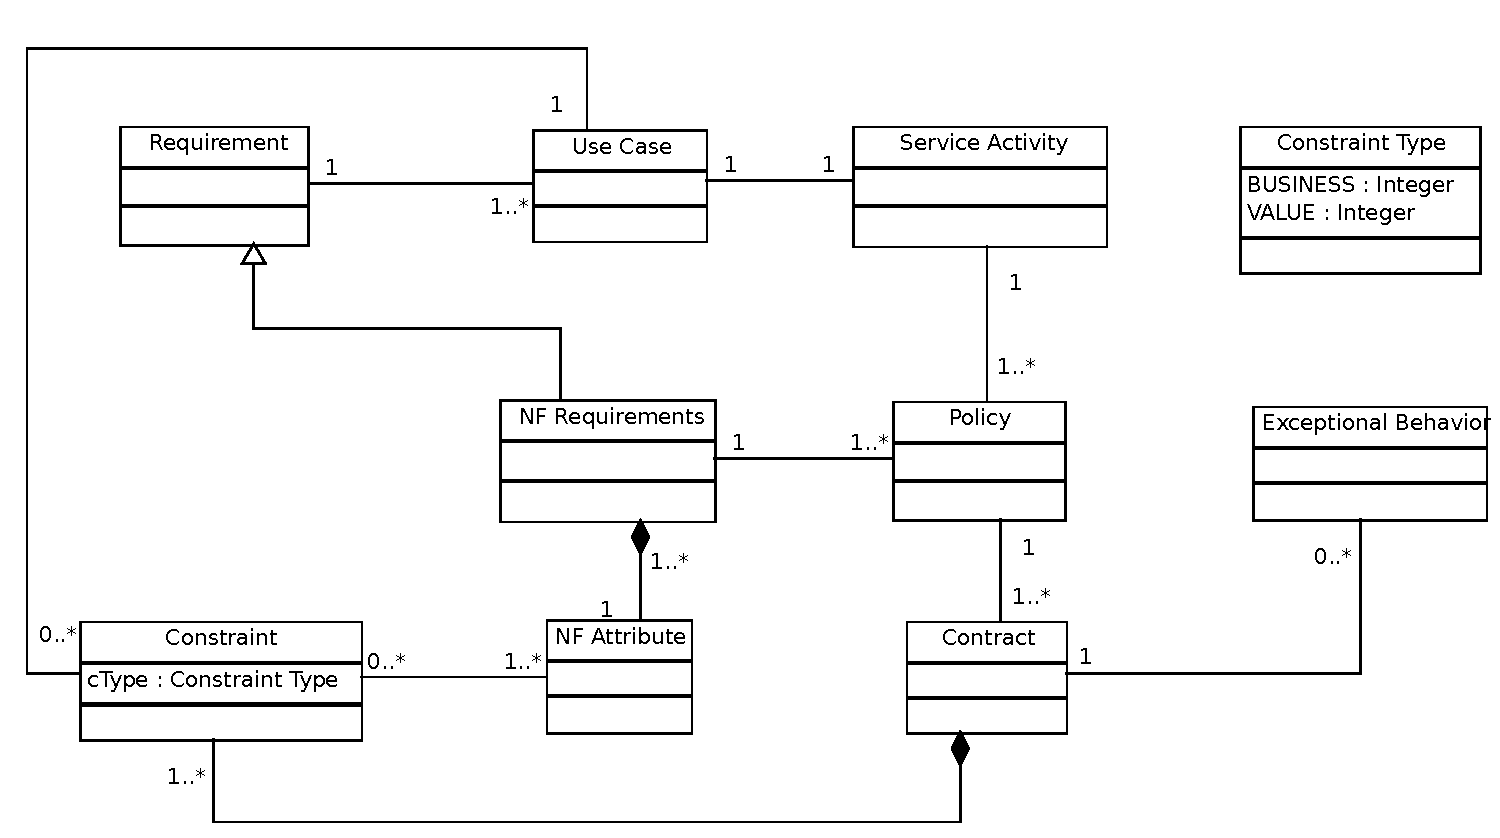
\includegraphics[width=0.70\textwidth]{figs/contractModel.pdf}
\caption{Service-Based Non-Functional Requirement Model.}
\label{fig:NRFmodel} 
\end{figure*} 

 \subsection{NFR Meta-Model} 
\label{sec:nfr-metamodel}



The model present in figure \ref{fig:NRFmodel} shows the relationship between
those concepts
%\footnote{The appendix
%\ref{app:nfr-concepts} provides a description of each concept presented in
%figure \ref{fig:NRFmodel}.} 
we consider important for quality requirements used
in service-based development.

% One requirement, whether functional or non-functional, can be represented by one
% or more use cases. For example, a paying process can be modeled through the use
% cases that represent withdrawal and deposit of money in transaction of customer
% and service provider accounts. A payment process also requires the guarantee of
% a complete transaction and data security. Thus several use cases are modeled to
% a single requirement. 

%Each concept represents:


One \texttt{Requirement}, whether functional or non-functional, can be
represented by one or more use cases. 
Each use case represents a \texttt{Service
Activity}. 
For example, a paying process can be modeled through the use cases
that represent withdrawal and deposit of money in transaction of customer and
service provider accounts. A payment process also requires the guarantee of a
complete transaction and data security. Thus several use cases are modeled to a
single requirement. All these use case can be implemented as services.
% 
% A composite use case is a type of use case. This type of
% use case abstracts a more macro function, and may contain extra functions to be
% performed so that the process is complete. For example, to publish a song, you
% must choose which song you want to publish, , authenticate to twitter or facebook,
% so that the music you're listening is published. We consider this type of use
% case, a use case compound.
 
Each use case has \textit{business} or
\textit{value} constraints. \textit{Business constraints} are restriction on
functions and how they may be implemented. The \textit{value constraints} are restrictions on
the service interface, which the desired values for input and output data. Each
constraint is associated with NFAs.

A \texttt{Contract} is a set of constraints for the same function. For example,
a contract for the payment operation. The constraints for payment are: (i) the
value amount should not be less than 10 euros and (ii) the user should always
receive a purchase confirmation by phone message. This restrictions are
grouped into a single contract for payment verification. 

% These constraints
% are also associated with non-functional attributes, e.g., reliability,
% transactions and data privacy card.
 
An \texttt{Exceptional Behavior} happens when a contract is not respected. When
this happens a new function is called or the process is stopped. For example, if
the bank does not authorize the payment, the system offers alternative forms
of payment such as PayPal.

Finally a \texttt{Policy} groups similar contracts. For example, security
contracts are grouped into a security policy and performance contracts are
grouped into a performance policy.


\subsection{NFR Classification}
\label{sec:nfr-classification}

 
\begin{figure*}[ht!]  
\centering  
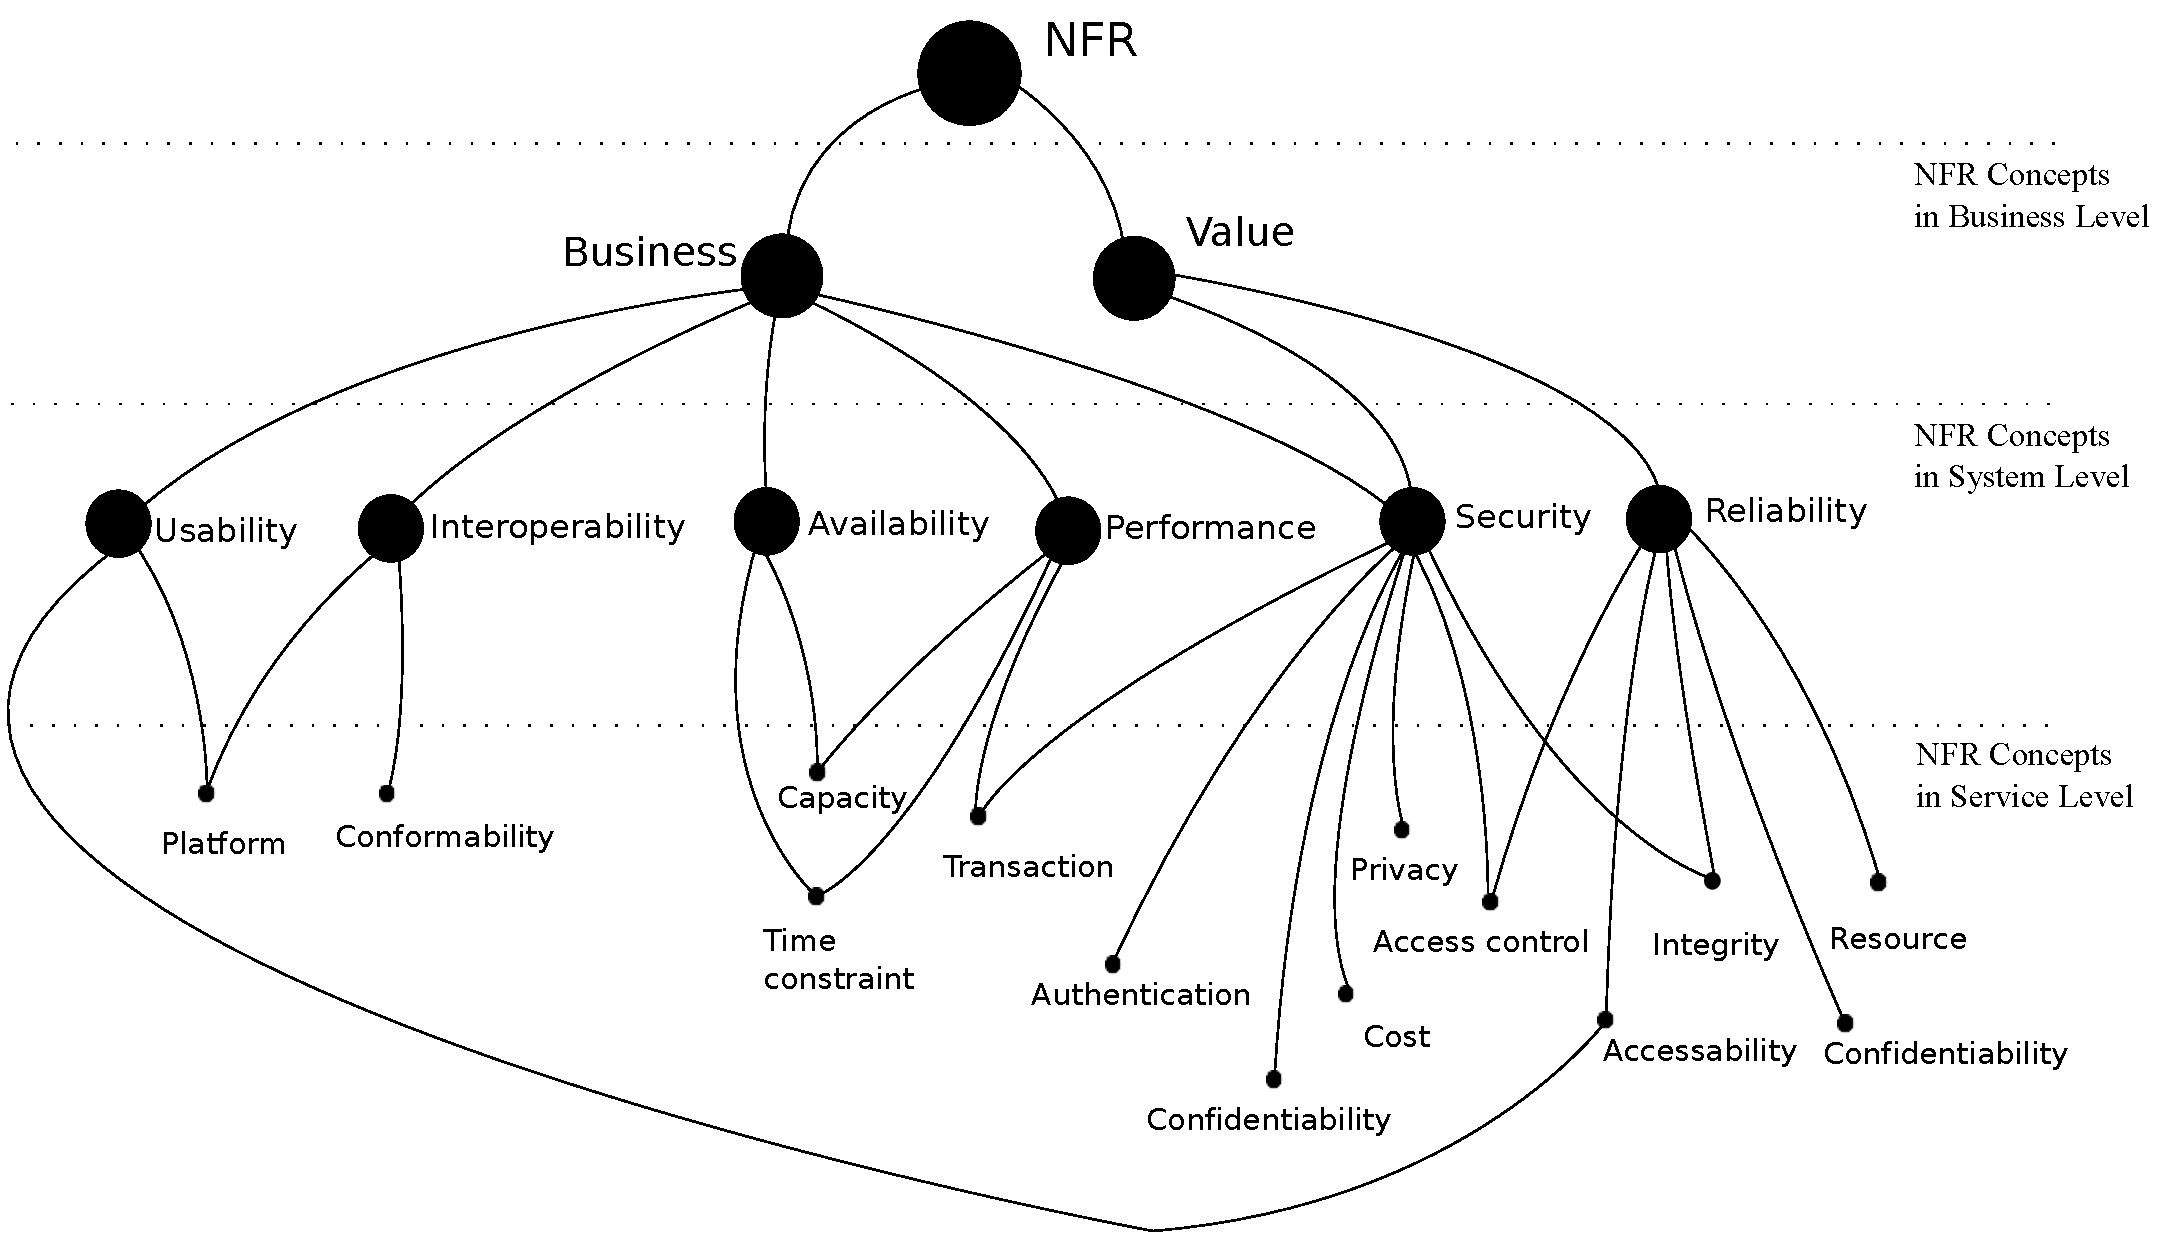
\includegraphics[width=0.70\textwidth]{figs/nfrRelationship.pdf}
\caption{Relationship of the NFR Concepts.}
\label{fig:nfr-relationship}   
\end{figure*}  

Table \ref{tab:result04} shows the NFR classification we propose, organized
 as follows (by column): (i) the level of abstraction, (ii) the proper term for
 this kind of abstraction and (iii) possible values to be used. The rows
 represent the abstraction level for modeling the NFR. The highest level is the
 \textit{Business level}, the intermediary one is the \textit{Service level};
 and finally the lowe level, called \textit{System level}.  
 
 
 

\begin{table}[ht!]
\centering
%\scriptsize
\tiny
\begin{tabular}{l|l|l}
  \hline 
  \hline
   \textbf{Modeling Level} & \textbf{\textit{Concept / Notation}} & \textbf{\textit{NFR / NFA}}  
   \\
  \hline
  \hline   
  Business Level & Constraint  & Business Constraint,    
 \\  
  &   & Value Constraint\\
   \hline    
   &  & Integrity, Transaction,  \\
   &  & Accessibility, Encryption, \\
   &  & Cost, Time Constraint, \\
  Service Level & Contract & Encryption, Platform, \\
   &  & Privacy, Authentication, \\
   &  & Resource, Capacity, \\
   &  & Privacy, Confidentiability 
   \\   \hline
   &  & Security, Performance,\\ 
   & & Interoperability, Scalability,\\
  System Level & Policy & Reliability, Usability,\\
   & & Transactional Behaviour,\\
   & & Availability \\ 
   \hline
  \hline  
\end{tabular}
\caption{Non-Functional Requirements Classification.}
\label{tab:result04}
\end{table} 


At the business modeling level, non-functional requirements are classified
into business restrictions. We have adopted, \textit{business} and \textit{value}
constraints to address the most abstract levels of restrictions in business
modeling. 

 



The relationship between non-functional requirements and attributes help
identify groups of restrictions and contracts to develop specific policies. The
level of service shows non-functional requirements, and system level presents a
finer granularity, describing the non-functional attributes. Thus, a set of
contracts that are related to the same attribute form specific policies for the
system. The relationship between the concepts in business, service and system
levels are presented in figure \ref{fig:nfr-relationship}.


% \begin{itemize}
%   \item Security:
% 	\begin{itemize}
%   		\item Access control; Transaction; Privacy; Cost; Authentication;
%   		Integrity; and Confidentiability.
% 	\end{itemize}
%   \item Performance:
% 	\begin{itemize}
%   		\item Time constraint; Capacity; and Transaction.
% 	\end{itemize}
% 	\item Availability:
% 	\begin{itemize}
%   		\item Capacity; and Time constraint.
% 	\end{itemize}
% 	\item Interoperability:
% 	\begin{itemize}
%   		\item Conformability; and Platform.
% 	\end{itemize}
% 	\item Usability: 
% 	\begin{itemize}
%   		\item Accessibility; and Platform.
% 	\end{itemize}
% 	\item Reliability:
% 	\begin{itemize}
%   		\item Access control; Confidentiability; Accessibility; Integrity; and
%   		Resource.
% 	\end{itemize}
% \end{itemize}

In our work we adopt \textit{security, performance, availability,
interoperability, usability} and \textit{reliability} as NFRs (these are
system level properties), and we consider as NFAs \textit{access control, time
constraint, privacy, accessibility} and so on (which are service level
properties).


\section{Conclusions}
\label{sec:conclusion}
 
 
This paper presented a systematic review of NFRs associated with web services.
We grouped the NFRs according to their characteristics and analyzed them in each
context of application. We also reviewed some existing NFR classification for service-based
development.
% In general, after reviewing the current research works related
% with the problem of service-oriented development, we could obtain
% some conclusion. 

To the best of our knowledge, there are no proposals that define a
service-oriented approach for the \textit{complete} development of systems,
considering non-functional requirements. Although many efforts have been made to support the new
technological proposals for the Web such as web services, in general, existing
approaches focus their processes on traditional software engineering
methodologies, with emphasis to the functional aspects of the application.

Thus, our analysis and classification can help to improve the development of
service-based applications which have as their main effort the
guarantee of quality requirements and the generation of reliable systems,
considering NFRs. We believe that the early modelling of NFRs during the
software process helps users and developers to improve the quality of the
solution.
   
\bibliographystyle{abbrv}
\bibliography{biblio} 
\end{document}
